% =============================================================================
%  template bits (c) 2014 Daniel Thau (paradigm)
%  modifications (c) 2014 Chris Wallace, both under the Apache v2 license
% =============================================================================

\documentclass[aspectratio=1610]{beamer}                  % beamer class, good for slides

\usepackage[T1]{fontenc}                % use a modern scalable font
%\usepackage{arev}                     % Helvetica
\usepackage{fontspec}
\setmainfont{Droid Sans}

\usepackage{amsmath}

\usepackage{xifthen}                    % \ifthenelse
\usepackage{listings}                   % code formatting
\usepackage{tikz}                       % vector drawing
\usepackage{booktabs}                   % fancy tables
\usepackage{varioref}                   % fancy cross referencing
\usepackage{xr-hyper}

\usetheme{CambridgeUS}
\beamertemplatenavigationsymbolsempty    % remove nav symbols

% - - - - - - - - - - - - - - - - - - - - - - - - - - - - - - - - - - - - - - -
%  theme color settings
% - - - - - - - - - - - - - - - - - - - - - - - - - - - - - - - - - - - - - - -
% drive, drive on down that field, men of the scarlet and gray!
\definecolor{OSUscarlet}{RGB}{187,0,0}
\definecolor{OSUgray}{RGB}{102,102,102}
% above values directly from brand.osu.edu/color

% change color for assorted sections
\setbeamercolor{description item}{fg = OSUscarlet}
\setbeamercolor{itemize item}{fg = OSUscarlet}
\setbeamercolor{itemize subitem}{fg = OSUgray}
\setbeamercolor{enumerate item}{fg = OSUscarlet}
\setbeamercolor{section in toc}{fg = OSUscarlet}
\setbeamercolor{subsection in toc}{fg = OSUgray}

% change color for assorted sections
\setbeamertemplate{section in toc}[default]
\setbeamertemplate{subsection in toc}[default]
\setbeamertemplate{itemize item}{\scriptsize\raise1.25pt\hbox{\donotcoloroutermaths$\blacktriangleright$}}
\setbeamertemplate{itemize subitem}{\tiny\raise1.5pt\hbox{\donotcoloroutermaths$\blacktriangleright$}}
\setbeamertemplate{itemize subsubitem}{\tiny\raise1.5pt\hbox{\donotcoloroutermaths$\blacktriangleright$}}
\setbeamertemplate{enumerate item}{\insertenumlabel.}
\setbeamertemplate{enumerate subitem}{\insertenumlabel.\insertsubenumlabel}
\setbeamertemplate{enumerate subsubitem}{\insertenumlabel.\insertsubenumlabel.\insertsubsubenumlabel}
\setbeamertemplate{enumerate mini template}{\insertenumlabel}

% - - - - - - - - - - - - - - - - - - - - - - - - - - - - - - - - - - - - - - -
%  theme frame settings
% - - - - - - - - - - - - - - - - - - - - - - - - - - - - - - - - - - - - - - -
%
% adjustment of the header to feature the title instead of defaults
\setbeamertemplate{headline}
{
	\leavevmode%
	\hbox{%
		\begin{beamercolorbox}[wd=.5\paperwidth,ht=2.25ex,dp=1ex,right,rightskip=1em]{section in head/foot}%
			\usebeamerfont{subsection in head/foot}\hspace*{2ex}\insertshorttitle
		\end{beamercolorbox}%
		\begin{beamercolorbox}[wd=.5\paperwidth,ht=2.25ex,dp=1ex,left,leftskip=1em]{subsection in head/foot}%
			%	\usebeamerfont{section in head/foot}\insertsectionhead\hspace*{2ex}
	\end{beamercolorbox}}%
	\vskip0pt%
}

% adjustment of the footer to an organization name instead of defaults

\setbeamertemplate{footline}{
	\leavevmode%
	\hbox{%
		\begin{beamercolorbox}[wd=.4\paperwidth,ht=2.25ex,dp=1ex,center]{author in head/foot}
			\usebeamerfont{author in head/foot}
			\insertorgname
		\end{beamercolorbox}%
		\begin{beamercolorbox}[wd=.6\paperwidth,ht=2.25ex,dp=1ex,right]{title in head/foot}
			\usebeamerfont{title in head/foot}
			\insertdate \hspace*{2em}
			\insertframenumber{} / \inserttotalframenumber\hspace*{3ex}
	\end{beamercolorbox}}
	\vskip0pt
}
% - - - - - - - - - - - - - - - - - - - - - - - - - - - - - - - - - - - - - - -
%  code result environment
% - - - - - - - - - - - - - - - - - - - - - - - - - - - - - - - - - - - - - - -
%
% code is often paired with there result, but has to be entered outside of
% frame.  use code from outside frame (\code), paired with result
%

\newenvironment{coderesult}{
	\begin{block}{Code}      % block, called Code
		\code                % print \code
	\end{block}
	\begin{block}{Result}    % block, called Result
	}{                           % result argument is here
	\end{block}
}

% - - - - - - - - - - - - - - - - - - - - - - - - - - - - - - - - - - - - - - -
%  section slide command
% - - - - - - - - - - - - - - - - - - - - - - - - - - - - - - - - - - - - - - -
%
% new command to draw a simple line.  it will be as long as available,
% and 1pt wide.  used for some stylizing
%

\newcommand{\srule}{
	\rule{\textwidth}{1pt}\\
}

% - - - - - - - - - - - - - - - - - - - - - - - - - - - - - - - - - - - - - - -
%  section break command
% - - - - - - - - - - - - - - - - - - - - - - - - - - - - - - - - - - - - - - -
%
% new command to create a title page for a particular section
%

\newcommand{\sectionslide}[1]{
	\begin{frame}
		\Huge
		\begin{center}
			#1
		\end{center}
	\end{frame}

}
% - - - - - - - - - - - - - - - - - - - - - - - - - - - - - - - - - - - - - - -
%  custom slide environment
% - - - - - - - - - - - - - - - - - - - - - - - - - - - - - - - - - - - - - - -
%
% essentially frame, but automatically adds section and possibly subsection as
% title.  also increases default font size
%
% method to detect subsection presence is kind of hacky:
% find it's width. if it has any width, it exists.
%

% variable to hold subsection's width
\newlength{\subsecwidth}

% slide environment - frame, plus automatic title
\newenvironment{slide}{
	\begin{frame}                                    % frame
		\settowidth{\subsecwidth}{\insertsubsection} % find subsection width
		\ifthenelse{\dimtest{\subsecwidth}{<}{1pt}}{ % no subsection
			\frametitle{\huge \insertsection\\             % insert *just* section
				\vspace{-1ex}                            % move next line up a bit
				%\color{fore}\srule                       % pretty line
				%\par                                     % remove excess spacing
				%\vspace{-3ex}                            % remove excess spacing
			}
		}{                                           % subsection exists
			\frametitle{\huge \insertsection\ -- \insertsubsection\\ % sec - subsec
				\vspace{-1ex}                            % move next line up a bit
				%\color{fore}\srule                       % pretty line
				%\par                                     % remove excess spacing
				%\vspace{-3ex}                            % remove excess spacing
			}
		}
		\Large                                       % make font in slide Large
	}{
	\end{frame}
}

% \frame needs [fragile] to handle lstlisting, but setting this is funky.  \fslide is a work-around

% variable to hold subsection's width
\newenvironment{fslide}{
	%\begin{frame}[fragile]
	\settowidth{\subsecwidth}{\insertsubsection} % find subsection width
	\ifthenelse{\dimtest{\subsecwidth}{<}{1pt}}{ % no subsection
		\frametitle{\insertsection\\             % insert *just* section
			\vspace{-1ex}                            % move next line up a bit
			\color{fore}\srule                       % pretty line
			\par                                     % remove excess spacing
			\vspace{-3ex}                            % remove excess spacing
		}
	}{                                           % subsection exists
		\frametitle{\insertsection\ -- \insertsubsection\\ % sec - subsec
			\vspace{-1ex}                            % move next line up a bit
			\color{fore}\srule                       % pretty line
			\par                                     % remove excess spacing
			\vspace{-3ex}                            % remove excess spacing
		}
	}
	\Large                                       % make font in slide Large
}{
	%\end{frame}
}

% - - - - - - - - - - - - - - - - - - - - - - - - - - - - - - - - - - - - - - -
%  title page
% - - - - - - - - - - - - - - - - - - - - - - - - - - - - - - - - - - - - - - -
%

\newcommand{\titleslide}[1]{
	\section{#1}             % set the section based on argument
	\begin{slide}
		\begin{center}
			\color{comments}
			\Huge            % Huge font size
			#1               % print new section's title
		\end{center}
	\end{slide}
}

% - - - - - - - - - - - - - - - - - - - - - - - - - - - - - - - - - - - - - - -
%  formatting commands
% - - - - - - - - - - - - - - - - - - - - - - - - - - - - - - - - - - - - - - -

%\renewcommand{\thefootnote}{\fnsymbol{footnote}} % fancy symbols for footnotes
%\newcommand{\cmd}[1]{\texttt{#1}} % fancy symbols for footnotes
% place at end of slide/frame to disable beamer vertical alignment
\newcommand{\disablevertalign}{\vskip0pt plus 1filll}

% - - - - - - - - - - - - - - - - - - - - - - - - - - - - - - - - - - - - - - -
%  title block
% - - - - - - - - - - - - - - - - - - - - - - - - - - - - - - - - - - - - - - -

\title{Vim: The Visual Editor}			% title
\author{Seattle Coder Dojo}
\date{Week 1}							% date
\newcommand{\insertorgname}{
	Seattle Coder Dojo
}

% =============================================================================
%  actual document begins here
% =============================================================================

\begin{document}
% *Content* below is distributed under a Creative Commons
% Share-Alike attribution 4.0 license (CC BY-SA 4.0).

\begin{frame}                           % title slide
	\titlepage                          % title page (title, author, date)
\end{frame}

\section{Housekeeping}
\subsection{Prerequisites}
\begin{slide}
    \begin{itemize}
        \item Can you use the computer?
        \item Can you use the keyboard?

            \pause
        \item Awesome! You know all you need to know to start this class :)
    \end{itemize}
\end{slide}

\subsection{Serialized Class}
\begin{slide}
    In case you didn't know, this is a serialized class! That means:
    \begin{itemize}
        \item We will be having 5 classes in a row, each building on the other.
        \item Missing one class may cause you to fall behind and be very confused.
    \end{itemize}
    I will publish these presentations and any materials we have, but that's no
    substitute for being here :)
\end{slide}

\section{What is Vim?}
\begin{slide}
    Vim is a \textbf{Vi}sual text editor.
	\begin{itemize}
        \item Once upon a time, we had to edit our files looking at \textit{one line at a time}.
        \item It was a big deal when Vi (and then Vi Improved) came along.
	\end{itemize}
\end{slide}

\section{What is a text editor?}
\begin{slide}
    A text editor is a program that lets you edit \textit{plain text}.
    \begin{itemize}
        \item Plain text doesn't have size or shape- it's just characters.
        \item What's the difference between Notepad and Microsoft Word?
    \end{itemize}
\end{slide}

\section{Why use and learn Vim?}
\begin{slide}
    \begin{itemize}
        \item It's everywhere:
            \begin{itemize}
                \item Almost every computer you will work with in the industry has Vim.
                \item Most other forms of software even have \textit{vim mode}, we'll talk about this later.
            \end{itemize}
        \item It's efficient:
            \begin{itemize}
                \item Most software engineers spend more time \textit{editing} existing code than writing new code.
                \item Vim makes it easy to jump around files and get exactly where you want to go.
                \item You don't have to use the mouse, or even move your fingers from the main part of the keyboard.
            \end{itemize}
    \end{itemize}
\end{slide}

\section{The Coder Dojo Workspace}
\begin{slide}
    \begin{itemize}
        \item We're trying something new this year: a standard development environment
            across our classes called \textbf{Cloud9}.

        \item Cloud9 is a development environment offered by Amazon, which is free for
            students, without a credit card.

        \item In today's class, we're going to get this environment set up and then cover some basics.
    \end{itemize}
\end{slide}

\subsection{Create a Workspace}
\begin{slide}
    Follow the instructions in the handout (link at the end of presentation).
\end{slide}
\begin{slide}
    \begin{center}
        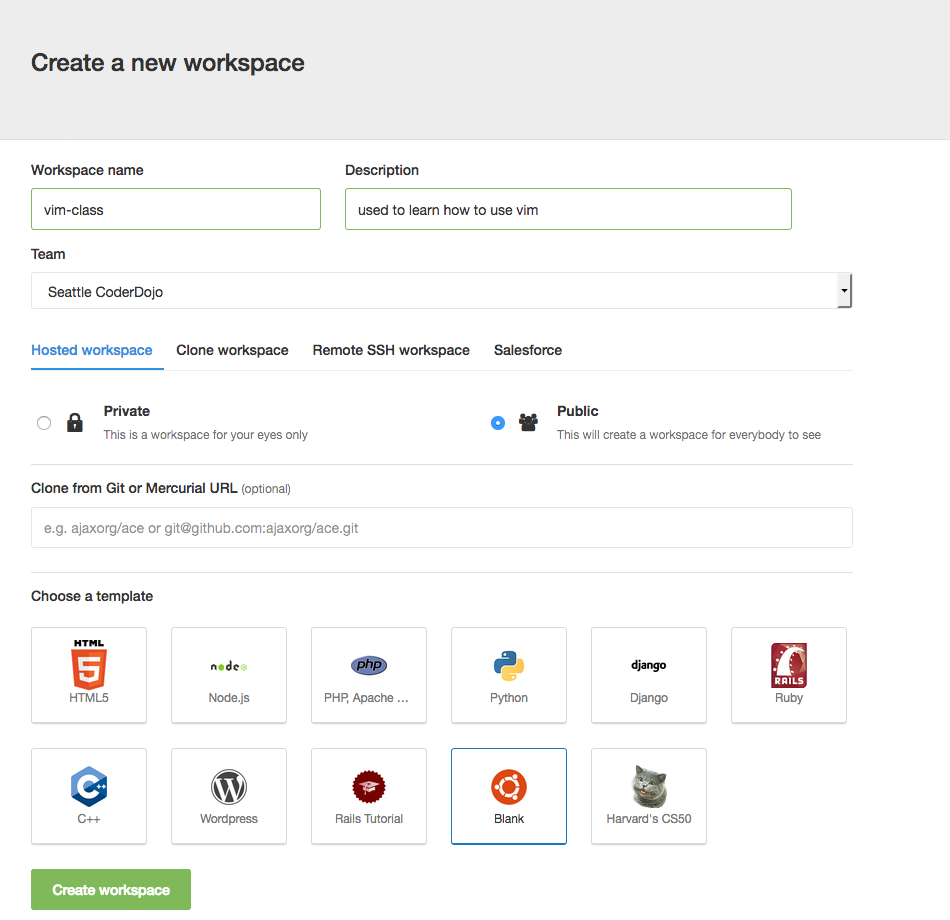
\includegraphics[width=0.5\textwidth]{images/workspace1}
    \end{center}
\end{slide}

\section{The Terminal}
\begin{slide}
    The Terminal, or \textit{Command Prompt}, is a prompt that accepts commands.
    \begin{itemize}
        \item This takes what you say and does them.
        \item The tricky part is, well, what do we type here?
        \item Let's try some things!
    \end{itemize}
\end{slide}

\subsection{\texttt{ls}}
\begin{slide}
    One of the most common things you need to do on a computer is see what
    files are in a folder.
    \begin{itemize}
        \item You could call this \textit{listing} a directory's contents.
        \item Let's try \texttt{ls}!
    \end{itemize}
\end{slide}

\subsection{\texttt{man}}
\begin{slide}
    What do you think this command does? What could it possibly be short for?
    \pause
    \begin{itemize}
        \item Manual pages!
        \item Let's try \texttt{man man}
     \end{itemize}
\end{slide}

\subsection{\texttt{cat}}
\begin{slide}
    What do you think this command does? Where could we find out?
    \pause
    \begin{itemize}
        \item \texttt{man cat}
        \item Concatenate is a fancy word that means ``link together''.
    \end{itemize}
\end{slide}

\subsection{Other commands to try}
\begin{slide}
        \begin{itemize}
            \item \texttt{cp}
            \item \texttt{mv}
            \item \texttt{pwd}
            \item \texttt{date}
            \item \texttt{cal}
            \item \texttt{uptime}
        \end{itemize}
\end{slide}

\subsection{Issuing Commands}
\begin{slide}
    When we issue commands, there are two main components:
	\huge
	\[
        \hspace {0em} \underbrace{\texttt{cp}}_{\text{command}}
        \underbrace{
        \hspace {1em}
            \texttt{README.md hi.md}
        \hspace {1em}
        }_{\text{arguments}}
	\]
\end{slide}

\begin{slide}
    \begin{itemize}
        \item The main idea behind the command prompt is that you specify what
            \textit{command} you want to run, first.
        \item Then, you provide anything you want that command to work on.
    \end{itemize}
\end{slide}

\section{Vim Basics}
\begin{slide}
    To open Vim, simply call it from the command line by typing, well, \texttt{vim}.
\end{slide}

\subsection{Modes}
\begin{slide}
    When you open vim, it's in something called \textbf{Normal Mode}.
    \begin{itemize}
        \item Normal mode is the normal, default mode vim is in.
        \item Try pressing the \texttt{i} key, then type.
            \begin{itemize}
                \item This is called \textbf{Insert Mode}. Notice the \texttt{-- INSERT --}
                \item These two mode are the main ones you'll work with in this class.
            \end{itemize}
        \item To return to normal mode, press Escape.
    \end{itemize}
\end{slide}

\subsection{Quitting}
\begin{slide}
    To quit vim:
    \begin{enumerate}
        \item Be in normal mode. If you're not, press Escape.
        \item Type \texttt{:q}
            \begin{itemize}
                \item Did that work? Why not?
                \item Try what it says: \texttt{:q!}
            \end{itemize}
    \end{enumerate}
\end{slide}

\subsection{Edit an Existing File and Scroll}
\begin{slide}
    How do you think we edit an existing file?
    \pause
    \begin{itemize}
        \item \texttt{vim README.md}
        \item In vim, we don't use the mouse or arrow keys. We instead use \textbf{H, J, K, and L}.
        \item Try it in normal mode! Get comfortable.
    \end{itemize}
\end{slide}

\subsection{Delete a character and Save}
\begin{slide}
    You can delete a single character with \texttt{x}.
    \begin{itemize}
        \item Can you remove all the exclamation marks and replace them with periods?
            \pause

        \item Save the file (but not quit) with \texttt{:w}
            \begin{itemize}
                \item \texttt{:wq} will save and quit
            \end{itemize}
    \end{itemize}
\end{slide}

\subsection{Insert vs Append}
\begin{slide}
    There are actually \textit{multiple ways} to get into insert mode. The two most popular are:
    \begin{itemize}
        \item \textbf{Insert} which is done with \texttt{i}
        \item \textbf{Append} which is done with \texttt{a}

        \item Can you spot the difference between the way these two behave?
    \end{itemize}
\end{slide}

\section{Links}
\begin{slide}
    \begin{itemize}
        \item The handout: \url{https://s3-us-west-2.amazonaws.com/notori0us/public/handout.pdf}
    \end{itemize}
\end{slide}
% link to more info
% link to this presentation
% link to handout

\end{document}
